\documentclass[9pt,aspectratio=169]{beamer}
\usetheme{CambridgeUS}
\usecolortheme{beaver}
\definecolor{nbycolor}{rgb}{0.6,0.17,0.8} % define color, named as nbycolor, use as: {colo
\usefonttheme{professionalfonts} % using non standard fonts for beamer
\usefonttheme{serif} % default family is serif
\usepackage{multirow}
\usepackage{array} % adjust table height
\usepackage{amsmath}
\usepackage{graphicx}
\usepackage{epstopdf}
\usepackage{animate}
\usepackage{media9}
\usepackage{ctex}
\setCJKmainfont{SimSun}
\setmainfont{Times New Roman}
% \title[Direct Integral Approach for Phase Transitions]{预测固体相变条件及状态方程的新方法---DIA}
\title[Direct Integral Approach for Phase Transitions]{DIA for Solid Phase transitions and Equations of State}
% \subtitle[]{--- \emph{SUBTITLE}}
\author[]{{\large \emph{Bo-Yuan Ning (宁博元)}}\inst{$^\dagger$}, {\Large \emph{Xi-Jing Ning (宁西京)}\inst{$^\ddagger$}}}
% \institute[byning@fudan.edu.cn, xjning@fudan.edu.cn]{
% \institute[宁博元, 宁西京$\cdot$复旦大学现代物理研究所]{
\institute[Bo-Yuan Ning, Xi-Jing Ning $\cdot$ IMP@FDU]{
  \inst{} {\large Institute of Modern Physics $\cdot$ Fudan University} \and
  \inst{$^\dagger$} \small{byning@fudan.edu.cn} \quad
  \inst{$^\ddagger$} \small{xjning@fudan.edu.cn}
}
% \date{\today}
% 
\date{CPS2022 $\cdot$ 深圳}
% \titlegraphic{
%   
\includegraphics[width=2cm]{../pics/FDU.png}
% }
\usepackage{tikz}
\titlegraphic{ 
\begin{tikzpicture}[overlay,remember picture]
\node[right=1cm] at (current page.160){
    
\includegraphics[width=1.1cm,height=1.1cm]{../pics/FDU}
};
\end{tikzpicture}
}
%   \logo{
% 
\includegraphics[width=3cm]{../pics/FDU.jpg}
% }
\begin{document}
\renewcommand\arraystretch{0.85} % height of table turnsto be 0.9 of default
% title-page
\begin{frame}
  \titlepage
\end{frame}
\section{\uppercase\expandafter{\romannumeral1}. 问题的提出}
\subsection{凝聚态体系的自由能$\mathcal F$和配分函数$\mathcal Z$？}
\begin{frame}[t]{Slide}
\end{frame}

\section{\uppercase\expandafter{\romannumeral2}. 求解配分函数的理论模型：DIA}
\subsection{重新诠释高维积分的意义}
\begin{frame}
  \frametitle[t]{积分意义的重新诠释}
  \begin{columns}
    \column{0.45\textwidth}
    \pause
    \begin{figure}
      \centering
      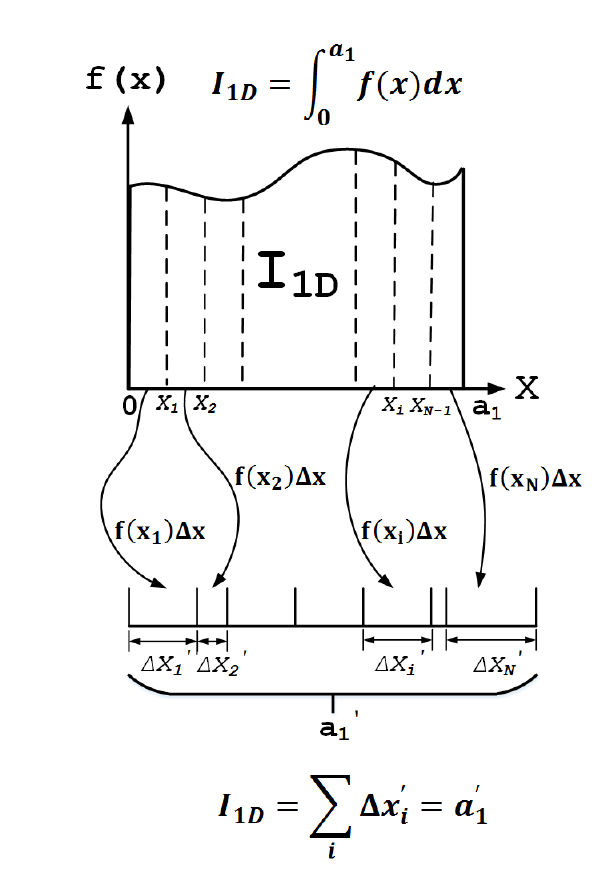
\includegraphics[height=1.5in, width=1.2in]{../pics/int1d}
    \end{figure}
      \centering
    \small{一维积分的重新诠释---等效长度}
    \column{0.45\textwidth}
    \pause
    \begin{figure}
      \centering
      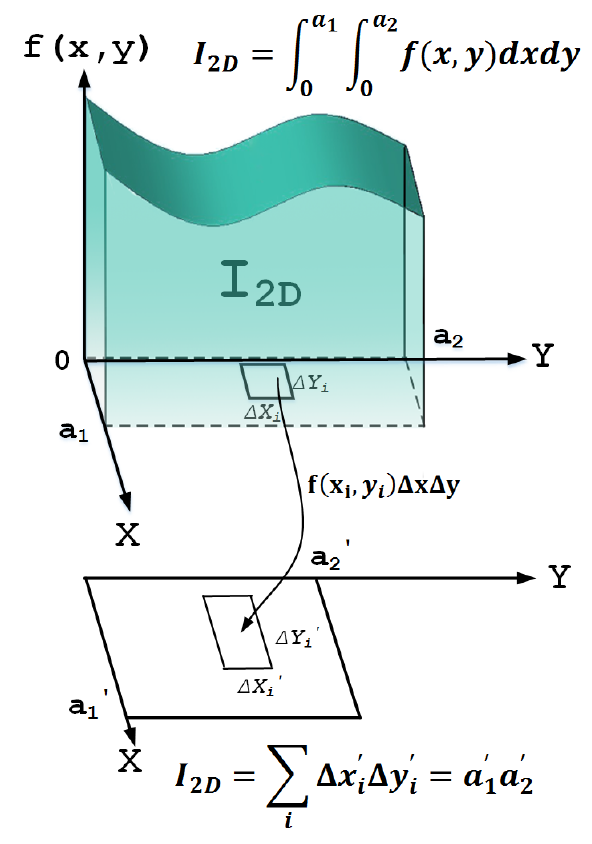
\includegraphics[height=1.5in, width=1.2in]{../pics/int2d}
    \end{figure}
      \centering
    \small{二维积分的重新诠释---等效面积}
  \end{columns}
    \pause
      \centering
      \center{$\downarrow$}\\
      \vspace{0.3cm}
      $N$维积分的重新诠释$\longrightarrow$ {\color{red} $N$维等效体积} \\
    \vspace{0.7cm}
      \footnotesize{\emph{Ning et al. J.Phys.:Conden.Matter \textbf{33}, 115901(2021)}}
      % \begin{block}{}{}
    % \end{block}

\end{frame}

\section{\uppercase\expandafter{\romannumeral3}. 应用DIA计算固体相变及状态方程}
\subsection{金属钒(V)}
\begin{frame}
  \frametitle[t]{Slide}
  \begin{columns}
  \end{columns}
\end{frame}
\subsection{金属铝(Al)}
\begin{frame}
  \frametitle[t]{Slide}
  \begin{columns}
  \end{columns}
\end{frame}
\subsection{金属锆(Zr)}
\begin{frame}
  \frametitle[t]{Slide}
  \begin{columns}
  \end{columns}
\end{frame}
\section{\uppercase\expandafter{\romannumeral4}. 总结与展望}
\begin{frame}
  \frametitle[t]{Slide}
  \begin{columns}
  \end{columns}
\end{frame}
\section{Appendix}


\end{document}

% columns
% \begin{columns}
%   \column{0.5 \textwidth}
%   \column{0.5 \textwidth}
% \end{columns}


% graphics
% \begin{figure}
%   \centering
%   \includegraphics[height=1.1in, width=0.5\textwidth]{}
% \end{figure}

% items
% \begin{itemize}
% \item item1
% \item item2
% \item item3
% \end{itemize}

% block
% \begin{block}{blocktitle}\vspace{1pt}
% \end{block}

% animate gif
% \animategraphics[width=\textwidth,autoplay,loop]{5}{pics/movegif/move-}{0}{60}

% movie, use movie15
% \begin{figure}
%   \includemovie[autoplay,loop]{1in}{1in}{figs/MD.avi}
% \end{figure}
